
\def\acmversion{}
%\def\mamversion{}
%\def\cmjversion{}
\def\finalversion{}

\def\continuousmapping{}
%\def\virtualmapping{}

\newlength{\baseimgwidth}	
\newlength{\basemapwidth}	

%--------------- using cmj template --------------
\ifdefined \cmjversion
\documentclass[letterpaper, 12pt]{article}

\usepackage{cmjStyle} %use CMJ style
\usepackage{natbib} %natbib package, necessary for customized cmj BibTeX style
\bibpunct{(}{)}{;}{a}{}{,} %adapt style of references in text
\doublespacing
\raggedright % use this to remove spacing and hyphenation oddities
%\setlength{\parindent}{0} % first para indent?
\setlength{\parskip}{2ex}
\parindent 24pt
\urlstyle{same} % make url tags have the same font
\setcounter{secnumdepth}{-1} % remove section numbering


%% The package endfloat moves all floats (figures, tables...) to the end of the paper, as required for the final version of a CMJ paper.
%% Leave this package commented out for initial submission, but uncomment it for final version. 
% \usepackage{endfloat}

\setlength{\baseimgwidth}		{0.6\columnwidth}
\setlength{\basemapwidth}		{1.6\baseimgwidth}
\def\mapsize{\footnotesize}

\fi


%--------------- using acm template --------------
\ifdefined \acmversion

\documentclass[10pt,twocolumn,acm]{article}

\textwidth = 6.5 in
\textheight = 9 in
\oddsidemargin = 0.0 in
\evensidemargin = 0.0 in
\topmargin = 0.0 in
\headheight = 0.0 in
\headsep = 0.0 in
\parskip = 0.2in
\parindent = 0.0in


\setlength{\baseimgwidth}		{\columnwidth}
\setlength{\basemapwidth}		{\columnwidth}
\def\mapsize{\scriptsize}

\usepackage[utf8]{inputenc}
\fi

%--------------- using jmam template --------------
\ifdefined \mamversion

\documentclass[]{tMAM2e}

\usepackage[utf8]{inputenc}
\usepackage{breqn}
\usepackage{pslatex}
\usepackage{verbatim}

\setlength{\baseimgwidth}		{\columnwidth}
\setlength{\basemapwidth}		{\baseimgwidth}
\def\mapsize{\small}

\fi

\usepackage{psfrag}
\usepackage{amsmath}
\usepackage{latexsym, amssymb}
\usepackage{graphicx}
\usepackage{color}
\usepackage{hyperref}
\usepackage{layout}


\definecolor{mycolor}{rgb}{0.384,0.0,0.145}
\hypersetup{
	colorlinks=true,
	linkcolor= mycolor,
	citecolor= mycolor
}

\definecolor{mygrey}{gray}{0.92}
\newcommand{\map}	[2]			{\begin{center}\colorbox{mygrey}{
								\begin{minipage}[t]{#1\basemapwidth} 
								{\mapsize \texttt{#2}}
								\end{minipage}}\end{center}}

\newcommand{\maptab}	[3]			{\begin{center}\colorbox{mygrey}{
								\begin{minipage}[t]{#1\basemapwidth} 
								{\mapsize 
								\vspace{#2}
								\texttt{\begin{center}
								\begin{tabular}{r@{ $\rightarrow$ }l}
								#3
								\end{tabular}
								\end{center}
								}}
								\end{minipage}}\end{center}}


\renewcommand{\baselinestretch}{1.175}
\makeatletter

\newcommand{\todo}	[1]			{{\big [\texttt{\textbf{#1}}]}}
\newcommand{\emptyseg}		{\ensuremath{\oslash}}
\newcommand{\raff}				{\ensuremath{\preccurlyeq}}
\newcommand{\domaine}			{{\mathcal Dom}}
\newcommand{\seg}[1]			{Seg(#1)}
\newcommand{\compose}			{*}
\newcommand{\lra}				{\ensuremath{\leftrightarrow}}
\newcommand{\variete}			{\ensuremath{\mathcal{V}}}
\newcommand{\fvariete}		{\ensuremath{[0,1[^{[0,1[}}}
\newcommand{\identite}		{\ensuremath{id}}
\newcommand{\semblable}		{\ensuremath{\equiv}}

\ifdefined \virtualmapping
\newcommand{\VDMapping}		{Virtual Mapping}
\newcommand{\vdmapping}		{virtual mapping}
\fi
\ifdefined \continuousmapping
\newcommand{\VDMapping}		{Continuous Mapping}
\newcommand{\vdmapping}		{continuous mapping}
\fi


\definecolor{commentcolor}{rgb}{1.,0.0,0.145}
\newcounter{comment}
\setcounter{comment}{1}
%\newcommand{\remark}[1]		{\textcolor{commentcolor}{\textbf{Comment \arabic{comment}: }}{\small \texttt{#1}} \addtocounter{comment}{1}}


\begin{document}

\ifdefined \mamversion

\doi{10.1080/1745973YYxxxxxxxx}
 \issn{1745-9745} \issnp{1745-9737}

  \jnum{00} \jyear{2011} \jmonth{January}

\markboth{Taylor \& Francis and I.T. Consultant}{Journal of Mathematics and Music}

\fi

%----------------- using CMJ template --------------
\ifdefined \cmjversion

%{\cmjTitle Segments and Mapping for Scores and Signal Representations}
{\cmjTitle Formalizing Segments and their Relationships in Music, Sound and Gestures Representations}
\vspace*{24pt}

\ifdefined \finalversion
%author - name
{\cmjAuthor Dominique Fober *, Frederic Bevilacqua \dag, Roland Assous \ddag}
%author - address
\newline
\begin{cmjAuthorAddress}
	* Grame - Centre national de cr\'eation musicale\\
	11 cours de Verdun Gensoul\\
	69002 Lyon, France\\
	fober@grame.fr \\
	\dag\ IRCAM \\
	1, place Igor-Stravinsky\\
	75004 Paris, France \\
	Frederic.Bevilacqua@ircam.fr
\end{cmjAuthorAddress}

\else
%author - address
{\cmjAuthor Firstname Lastname}
\newline
\begin{cmjAuthorAddress}
	Sound Computing Group\\
	University of Anywhere\\
	1234 Anywhere Street\\
	Anywhere, Anwhere 012345 USA\\
	email@email.com
\end{cmjAuthorAddress}

\vspace*{24pt}
{\cmjAuthorPhone << AUTHOR TELEPHONE (not for publication): +44 999 999 9999 >>}

\fi
\vspace*{24pt}

\section*{Abstract}
We present a general theoretical framework for a segmental approach in describing various musical, sonic and gestural elements.  Each segment can be related to different music representations, graphical scores, sound or gesture signals. Importantly, this theoretical formalism allows for the description of the relationships between the segments, called here \emph{mapping}, and thus deal with a large number of problems in music representations. We describe some examples of multimodal score representation where the symbolic score is superimposed with signal displays, in particular with gesture and sound signals.

%---------------- not using CMJ template -----------
\else

\title{\vspace{-5mm}
{\small \textsc {GRAME \\ 
Computer Music Lab.  \\}}
\vspace {-4mm}
{\normalsize Technical report TR-121213}\\
\vspace {4mm}
Segments and Mapping for \\Scores and Signal Representations}

\ifdefined \finalversion
\author{Dominique Fober$^{1}$, Frederic Bevilacqua$^{2}$, Roland Assous$^{3}$ \\
{\small \textit{$^{1}$GRAME - Lyon, $^{2}$IRCAM - Paris, $^{3}$Université Lyon 1}}}
\else
\author{author1, author2,...}
\fi
\date{}

\maketitle
\thispagestyle{empty}
\pagestyle{empty}

\abstract {We present a general theoretical framework to describe segments and the different possible mapping that can be established between them. Each segment can be related to different music representations, graphical scores, music signals or gesture signals. This theoretical formalism is general and is compatible with large number of problems found in sound and gesture computing. We describe some examples we developed in interactive score representation, superposed with signal representation, and the description of synchronization between gesture and sound signals.
}
\fi




\ifdefined \keywords
\keywords {interval, segment, segmentation, mapping, relationship }
\fi

%------------------------------------------------------------
\section{Introduction}
%------------------------------------------------------------

% segment and music, need for a general formalism
The explicit or implicit use of segments is necessary for the description of music. For example, elements such as notes, bars, sections can be considered as time segments. Beyond these obvious examples, symbolic and signal representations of music, including sound and gestures elements, do imply a large variety of segmental representations. Generally, the different applications, from musical notation to interactive system programing, make use of their own \emph{ad-hoc} formalisms. We argue here that a general formalism would facilitate the integration of different segmental approaches for both symbolic and signal music representations.  This should foster merging different computer music applications (or the communication between them), especially considering interactive sound systems dealing with graphical representations.
% complexity of relationships, non linearity

Music representation is  fundamentally not linear with respect to the time representation. The  possible relationships between the "dynamic time" of the performance and the time of the score can be complex, being potentially non-continuous and non-bijective. In music notation, repeat bars, jumps to \emph{segno} or \emph{coda} are some examples taken from the traditional western music notation, illustrating such a complexity. The dynamic  structure of jazz music poses similar issues, making automatic accompaniment a non-trivial task \cite{Gold2011,liang2011}.

%Similarly, the annotation of time based multimedia content requires to draw explicit relations between the multimedia graphic space and the time space. In \cite{Aubert:2005}, ADVENE, an hyper-video system is described, where the basic element of the model is the annotation, i.e. a piece of data linked to a part of an audiovisual document called a \emph{fragment}.
%, for example in the hyper-video domain \cite{Aubert:2005}.

%what about segment here ?

%extention to signal represenation 
Music representation, beyond the sole symbolic representation, should also include signal representation. In this regard, the problem of relationship we just mentioned should be generalized to the relationships between various classes of elements, symbol and signal segments. 

% ce paragraphe s'insère mal dans le flow....
For example, the classic case of Attack-Decay-Sustain-Release note representation in sound synthesis makes use of concatenated segments for control, that are related to sound processes. This could be generalize to more general gesture modeling in music performance, which can be segmented in preparation, stroke and release phases \cite{Francoise12a}. Formalizing relationships between such gesture and sound segments represents a current challenge in the design of interactive systems \cite{Bevilacqua2011Springer, Rasamimanana_OS09}. 

%goal of the paper
This paper proposes a simple but general formalism to describe time segments in various spaces. Specifically, we propose an explicit description of the relationships between segments. We will show in particular how this formalism can be used for a wide range of applications, and in particular in dynamic graphical scores and gesture-based interactive systems.

The paper is structured as follows. First, after a presentation of  related works, we describe the general problematics of time representations we tackle in this paper.  Second, we present our general framework for segments description and segmentation. Third, we describe a formal description of \emph{mappings} which is the term we'll use to refer to relations between segments, and fourth, how these mappings can be extended to \emph{\vdmapping s} using simple and intuitive operations. Fifth, we describe more advanced concepts of segments relationships, called \emph{refinement}. All the formal descriptions are accompanied by concrete examples of applications.

%------------------------------------------------------------
\section{Related Works}
%------------------------------------------------------------
% music notation, time representation
Let consider first the case of music notation. Music scores could be viewed as time representation: for most of the music representations, there is a more or less complex relationship between the graphical space of the notation and the performance time. Such relationships between the "music/performance time" and the music notation are made explicit in some applications.  

For example, in \cite{Fober:07b}, the authors discussed the relationship, in graphical space, between time representation in notation and in music performance. Intended to enhance music learning using a mirror metaphor, this work did not attempt to provide for a formal description of the relationship between time and graphic spaces,  being rather focused on specific required features for pedagogical applications. 

In \cite{bresson08}, the authors described a specific time representation, used in music composition tools such OpenMusic, to overcome issues arisen when combining different notation aspects with advanced time structures. An object called "sheet" is introduced in OpenMusic, providing a consistent graphical representation of different musical objects regarding their time dimension. This approach makes use of landmarks to compute ratios between time and space, that are gathered into a global discrete function $x=f(t)$. Nevertheless, this system is designed only for specific objects considering their time systems (e.g. proportional-time, continuous-time objects). It  cannot be generalized easily being based on a restricted formalism of time segments.



% on se répète ...
%While existing applications defines relationship between time and various instances or representations of time, there is a lack of explicit formalism, or algorithmic description of the underlying processes.

% state of the are:
%the representation problem: which one ?
Representing time relations was partially approached already in the early 90' by the HyTime proposal \cite{hytime91}, with the viewpoint of media synchronization but the HyTime initiative never succeeded \cite{sloan02}.
In some way, the SMIL specification \cite{hoschka98} could be viewed as the successor of HyTime: it is a recommended W3C XML markup language for describing multimedia presentations. Using SMIL, it is possible to describe the temporal behavior of a multimedia presentation, to associate hyperlinks with media objects and to describe the layout of the presentation on a screen.

Another approach has been proposed with the IEEE standard IEEE 1599 \cite{baggi09b}, which targets applications in which all aspects of music, such as audio and sound, graphical representation, historical data, performance indications, are fully integrated and synchronized. This standard specifies an XML description of multimedia resources, which are all related to an abstract time layer. It contains the necessary information to establish time relationships between various media using time as the \emph{spine} of the description. It is strongly anchored in the music domain and even provides users with a symbolic notational layer. 

% ????
Hence there are numerous approaches and formats to describe time relationships of which none succeeded in being widely supported. But above all, the existing approaches are mainly descriptive and lack of a formal description of the time relationships that enables a computational approach.

The recent extension of the music score by \cite{Fober:10c} led to a general formalism, covering the needs of media synchronization beyond the current state of the art. The synchronization issues are approached using  \emph{segmentation} and  relations between \emph{segments}. Similarly to previous approaches, time constitutes the spine of the system but the specification is independent of the media types and can be easily extended. The formalism we present in the next sections builds on this earlier work, describing a complete formal description of segment and their relationships.


%------------------------------------------------------------
\section{Problematics of time representations and their relationships}
%------------------------------------------------------------
%\remark{Cette section est \`a revoir, un peu trop simpliste... Fr\'ed\'eric sugg\`ere d'utiliser l'exemple de fin (fig.\ref{fig:gmapping-gesture-sound}) comme description de la complexit\'e attendue.}

\subsection{Music notation, annotation and \emph{time} space.}
%------------------------------------------------------------
Apart the purely graphic notations experiments conducted in the second half of the XX$^{th}$ century \cite{quist1984indeterminate,schnebel1969mo}, a music score generally establishes correspondences between the graphical space and the time space. 

For the sake of simplicity, most music applications using a score representation associate a single time position to a graphic position. Nevertheless, even simple music score might imply a graphical space of the music notation that is not organized proportionally to time (Fig. \ref{fig-repeat}).  For example, associating a staff to a single time interval generally leads to rough approximations of the actual relationship between time and the graphical space. To ensure accuracy to such a relationship, a finer segmentation of the graphical space is necessary, taking into account every symbol that can be associated to a time dimension.  Another common issue is due to the complex relationship existing between the notation and the dynamic time of the performance: this relationship is non-continuous and non-bijective, due to repeat bars, jumps (to \emph{coda}, to \emph{segno}...). Figure \ref{fig-repeat} illustrates the two issues we mentioned: non-proportionality between time and the graphical space and non-bijective relationship between notated and performed time.
\begin{figure*} %[htbp]
\begin{center}
	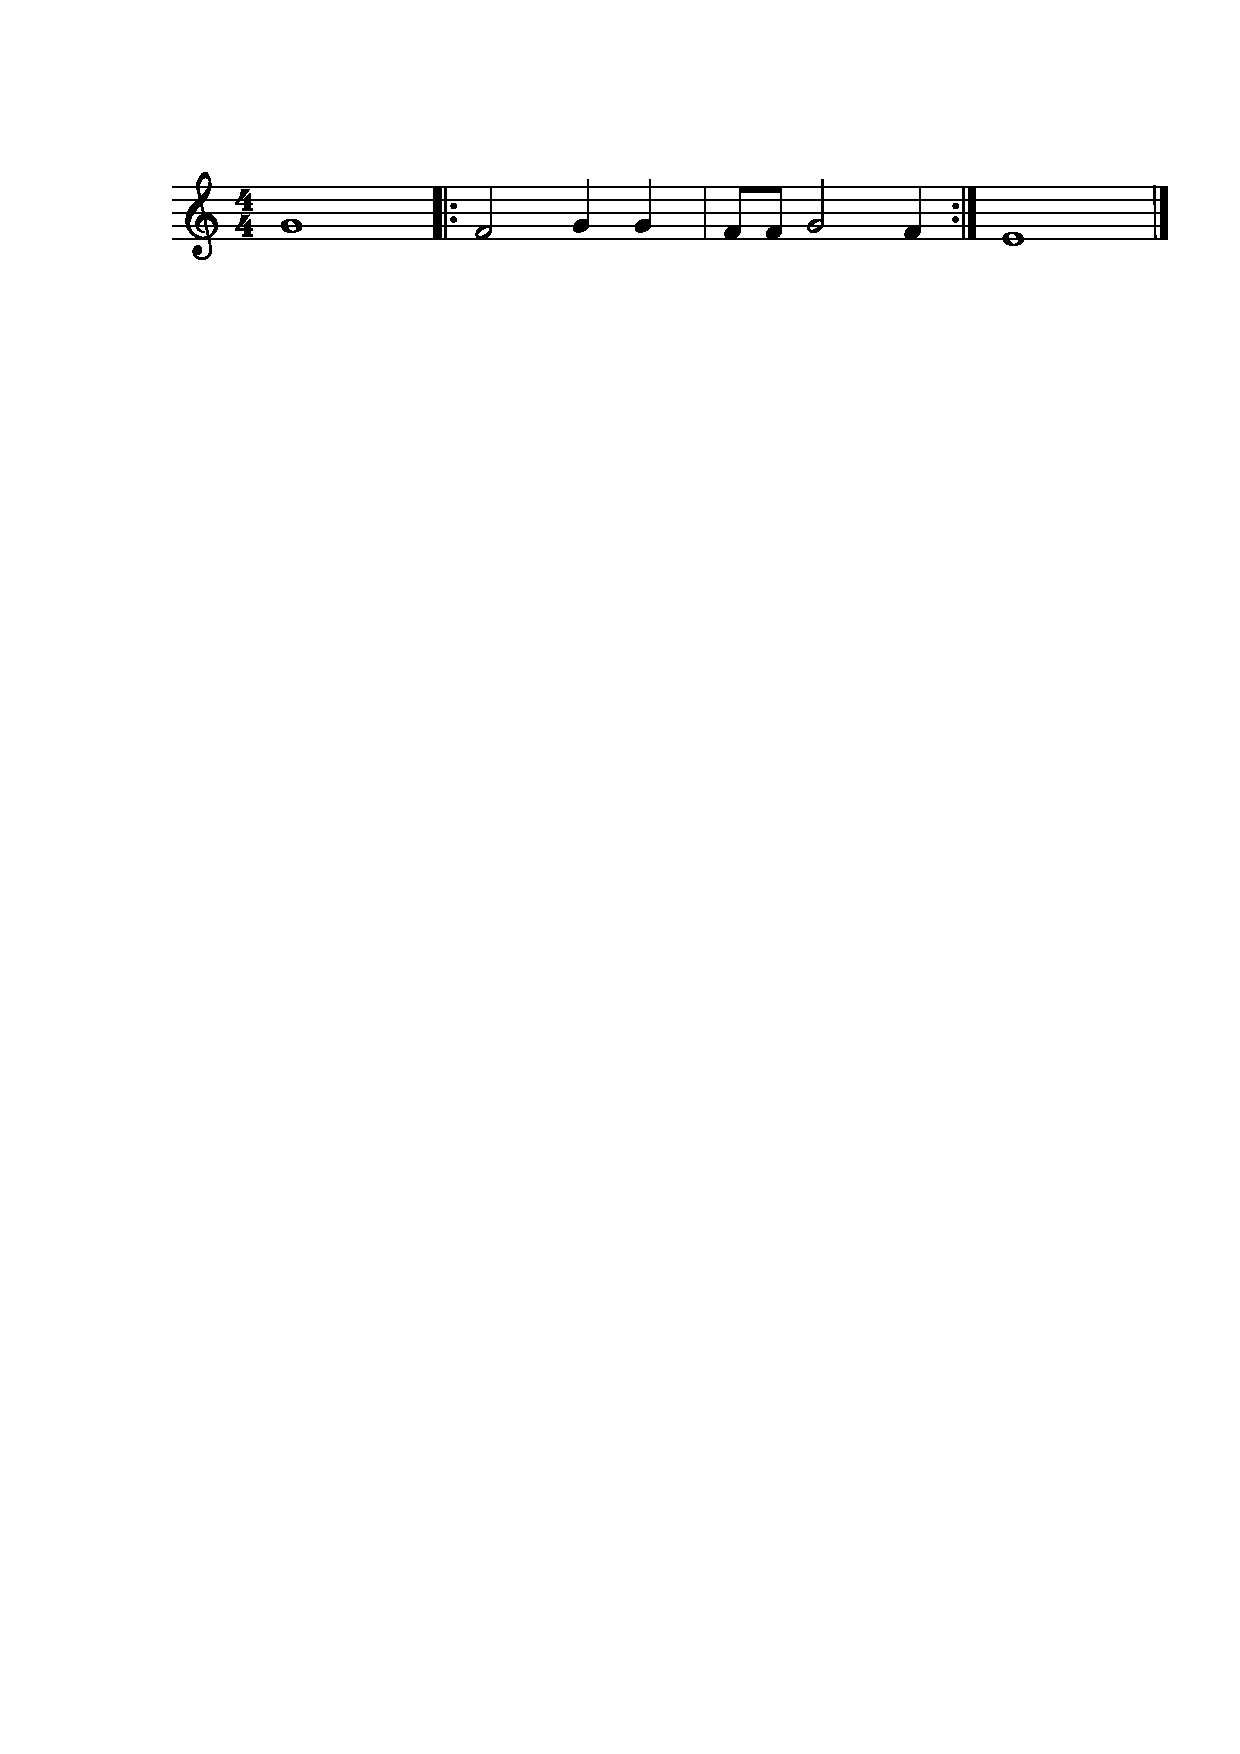
\includegraphics[width=1.3\baseimgwidth]{imgs/fig-repeat}
\caption{A music score illustrating two issues : non-proportionality between  time and the graphical space and non-bijective relationship between notated and performed time (due to repeated bars).}
\label{fig-repeat}
\end{center}
\end{figure*}


Music score annotation (e.g. a score annotated with textual data, or with a representation of its performance) is another case that requires an accurate relationship between time and space. 
%vers Dom
%Indeed, unless it concerns a static score, graphically instantiated and which layout is fixed, annotations should be made in the time domain while represented in the graphic domain.
%Indeed, for a static score, annotations could be associated to a graphic position, but for dynamic scores, they must be made in the time domain although represented in the graphic domain.
%vers Fred
In the case of static scores (typically printed), the annotation can be added directly to the graphic space without considering its precise time location, the choice of the graphical location being often constrained by readability issue. In the case of dynamic scores (e.g. interactive score), a more formal procedure must be established to guarantee consistency to changes, by taking into account a precise time for the annotation and for the graphical placement of annotation.
% PAS CLAIR 

Even more complex cases are found when the annotations have also a time dimension (e.g. a signal graphic representation). Figure \ref{fig-score-sig} shows an example of a music score and its performance represented as a graphic signal: a simple stretch of the performance image over the score cannot visually convey accurately the detailed time relationships between the score and the performance. 
\begin{figure} %[htbp]
\begin{center}
	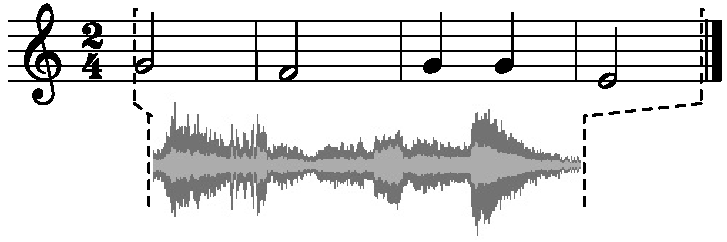
\includegraphics[width=0.9\baseimgwidth]{imgs/fig-score-sig3}
\caption{A music score with annotation consisting of a performance represented as a graphic signal. A simple stretch of the annotation would not suffice to represent accurately the  relationship between the score and the annotation. }
\label{fig-score-sig}
\end{center}
\end{figure}

\subsection{Describing time relationships in graphical space}
\label{sec:timetograph}
%------------------------------------------------------------

Beyond standard music scores, there is a need for a general system that can describe time relationships for arbitrary graphical objects. For example, it is useful to combine symbolic scores and various signal representations of sound and gesture elements. 
% (i.e. not score centered)  ???
This becomes especially important for interactive systems, where these relationships are dynamic, as their graphical representations. We present below two different examples taken from actual interactive applications.

%------------------------------------------------------------
\begin{figure} %[htbp]
\begin{center}
	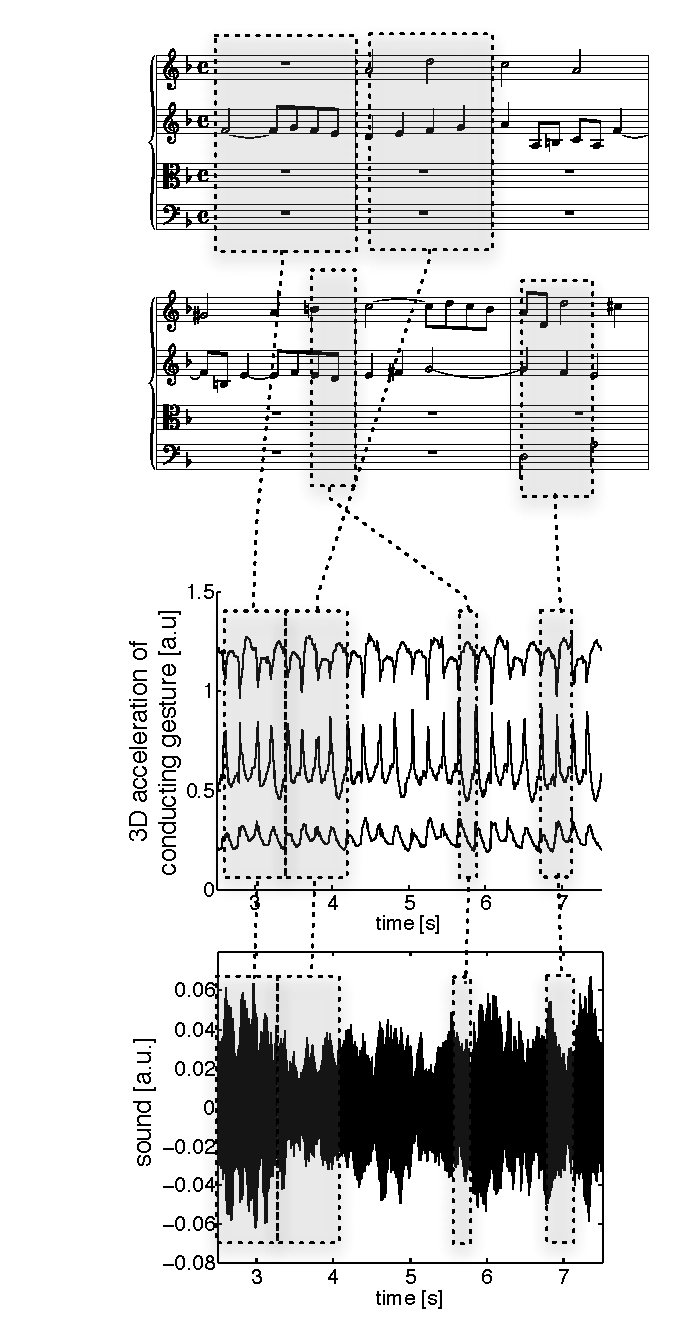
\includegraphics[width=\baseimgwidth]{imgs/fig-gesture-sound-segments}
\caption{Segments in score, sound and gesture signal representation. Case of conducting gestures, captured with 3D accelerometer, used to continuously control the pace of a recording.}
\label{fig:gesture-sound-segments}
\end{center}
\end{figure}


%------------------------------------------------------------
\begin{figure*} %[htbp]
\begin{center}
	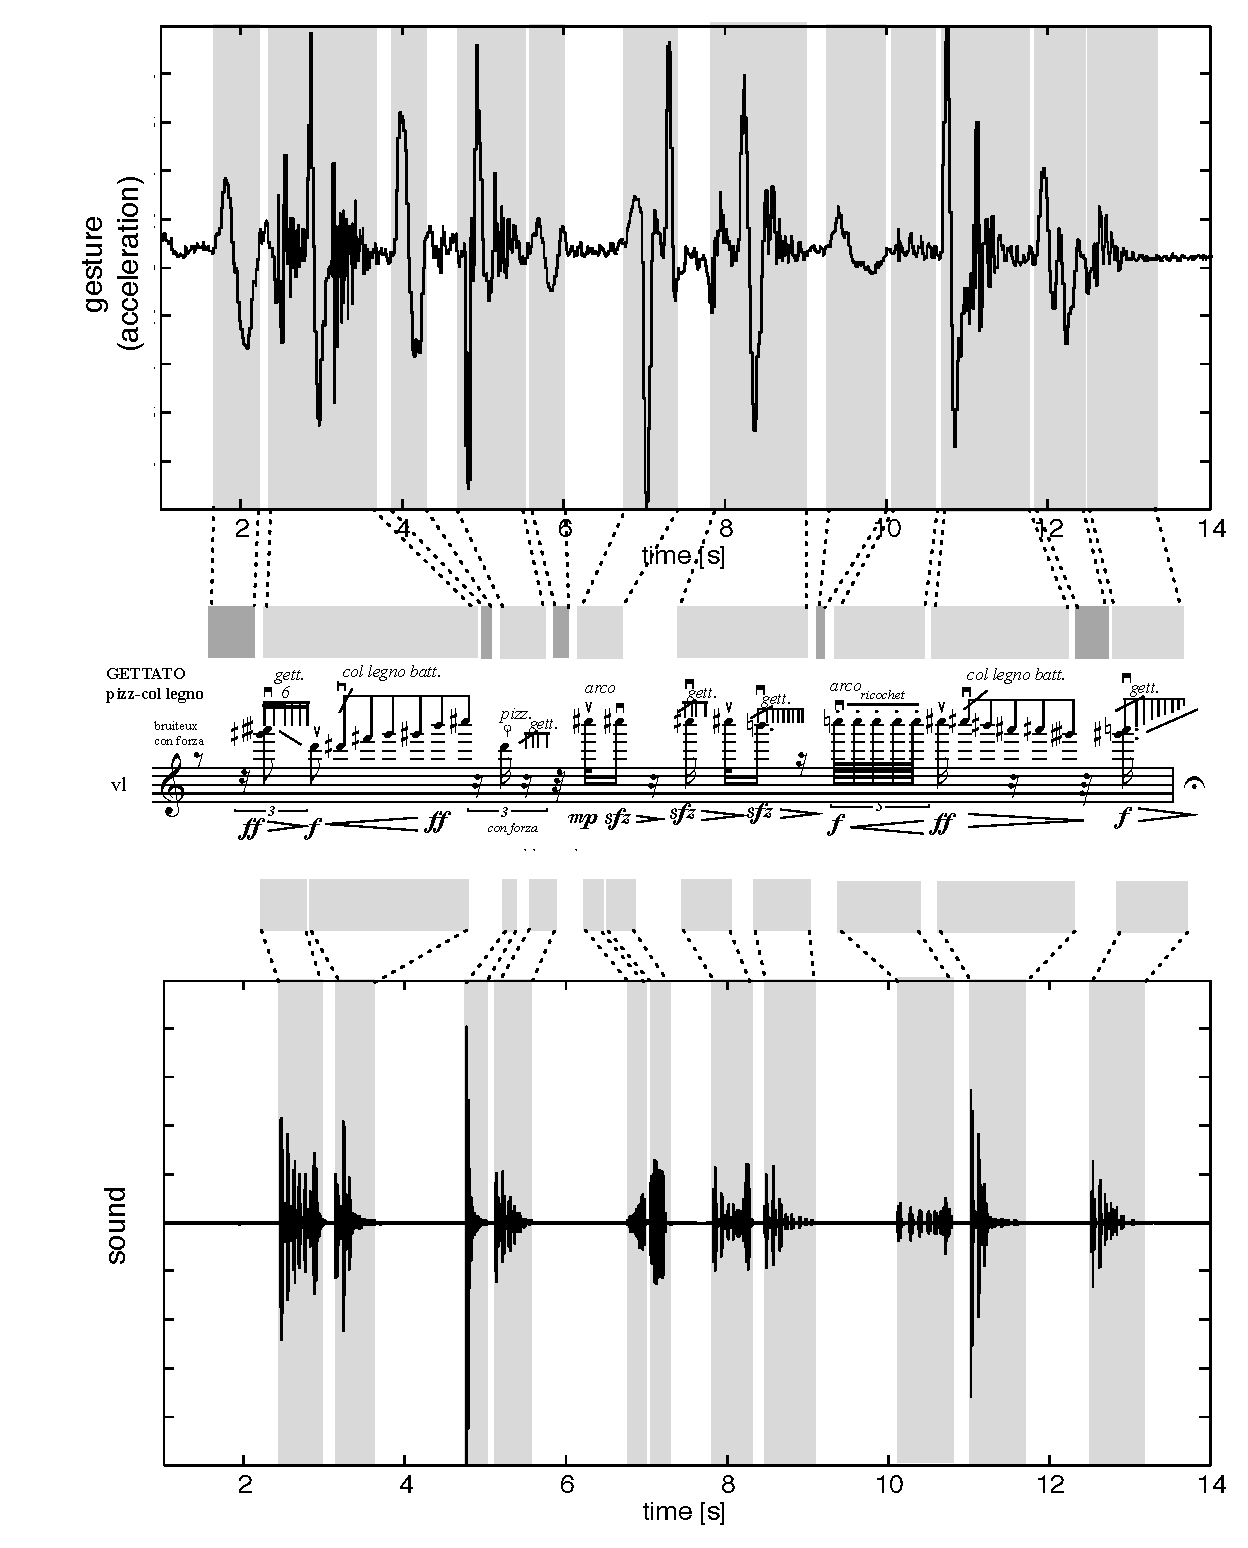
\includegraphics[width=1.5\baseimgwidth]{imgs/fig-mapping-gesture-sound4}
\caption{Relationship between different segmentation related to gesture or sound signals. Case of an augmented violin, where bow acceleration was recorded synchronously with the audio. Excerpt of the composition \emph{Streicherkreis} by Florence Baschet}.
\label{fig:gmapping-gesture-sound}
\end{center}
\end{figure*}

First, Figure \ref{fig:gesture-sound-segments} illustrates an example where temporal elements such as sound and gesture signal representations are linked to a symbolic score. The gesture signal here corresponds to the 3D acceleration of the hand of a conductor, displayed above the audio waveform. This case is taken from an existing pedagogical system \cite{bevilacqua_nime07} where a teacher or a student control the pace of an audio recording using "conducting gestures", captured with motion sensors. In such an application, it is vital to be able to visualize the symbolic scores synchronously with the signal representations, and to be allowed to draw direct links between them as indicated in Figure \ref{fig:gesture-sound-segments}.

Second, we present here an example taken from a series of experiments performed on an augmented quartet, where bow acceleration was measured synchronously with the sound \cite{Bevilacqua_JNMR2012}. Figure \ref{fig:gmapping-gesture-sound} displays the score, sound acceleration signals of a particular musical phrase. Interestingly, in this case the score includes relatively complex ornamentation, with no explicit time duration, which also exemplifies the complexity of the time relationships between symbolic and signals representations.

Figure \ref{fig:gmapping-gesture-sound} shows that gesture and sound signals can be segmented differently. The different forms of the signals naturally call for different segmentation strategies. 
First, the gesture signals includes gesture preparation signals that are segments not present in sound signals. Second, segments are typically of different durations for a given element of the symbolic score. Moreover, this might lead to different elements grouping, resulting finally in structurally different segmentations.

The next sections present the formalism that has been defined to handled the problematic described above. First,
segments and segmentations are formally defined. Then the notion of \emph{mapping} (i.e. relationship between segmentations) is introduced. Next, mappings are extended to \emph{continuous mapping}, which represents a way to draw relationships inside a segment. Finally, a \emph{refinement} operation is defined, that is used to build relationships between arbitrary segmentations.


%------------------------------------------------------------
\section{Segments and segmentations}
%------------------------------------------------------------

In this section we define the notions of \emph{segment} and \emph{ segmentation}. We will first introduce the notions of temporal and graphic segments. Next we will generalize these definitions for any abstract space. Finally, we introduce the notion of \emph{resource segmentation}, that is a necessary step to coherently define segment relationships within our formalism.


\subsection{Temporal Segment}
%----------------------------------------------------------------

A \emph{temporal segment} is defined as an interval 
 $i=[t_{0},t_{1}[$ such as $t_{0} \leqslant t_{1}$. The interval is empty when $t_{0} = t_{1}$ ; we will use the notation \emptyseg\  for empty intervals.

The intersection of two temporal segments (figure \ref{fig:segment1D}) $i_m$ and $i_n$ is defined by: 
$$ i_{m} \cap i_{n}  := \{ j \ |\ j \in i_m \ \land\ j \in i_n \} $$


\begin{figure} %[htbp]
\begin{center}
	\psfrag{t0}{$t_0$}
	\psfrag{t1}{$t_1$}
	\psfrag{t2}{$t_2$}
	\psfrag{t3}{$t_3$}
	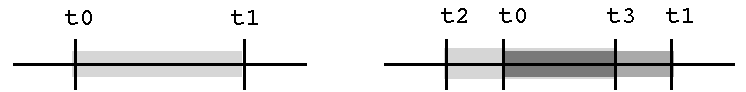
\includegraphics[width=0.9\baseimgwidth]{imgs/segments1DG}
\caption{from left to right: a temporal segment and the intersection of two temporal segments.}
\label{fig:segment1D}
\end{center}
\end{figure}


%----------------------------------------------------------------
\subsection{Graphic Segment}
%----------------------------------------------------------------
A \emph{graphic segment} (2D case) is defined as the product of two intervals $[x_0,x_1[$ et $[y_0,y_1[$ :
$$ [x_0,x_1[ \times [y_0,y_1[ := \{ (u,v) | u \in [x_0,x_1[ \land v \in [y_0,y_1[ \} $$

where $[x_0,x_1[$ is an interval on the abcissa and $[y_0,y_1[$, on the ordinate (figure \ref{fig:segment2D}).

A graphic segment $g = x \times y$ is empty when $x = \emptyseg $ or $y = \emptyseg $

The intersection operation $\cap$ between two graphic segments $g_{m}=x_{m} \times y_{m}$ and $g_{n}=x_{n} \times y_{n}$ is defined as :
$$ g_{m} \cap g_{n} := (x_{m} \cap x_{n}) \times (y_{m} \cap y_{n}) $$

\begin{figure} %[htbp]
\begin{center}
	\psfrag{x0}{$x_0$}
	\psfrag{x1}{$x_1$}
	\psfrag{y0}{$y_0$}
	\psfrag{y1}{$y_1$}
	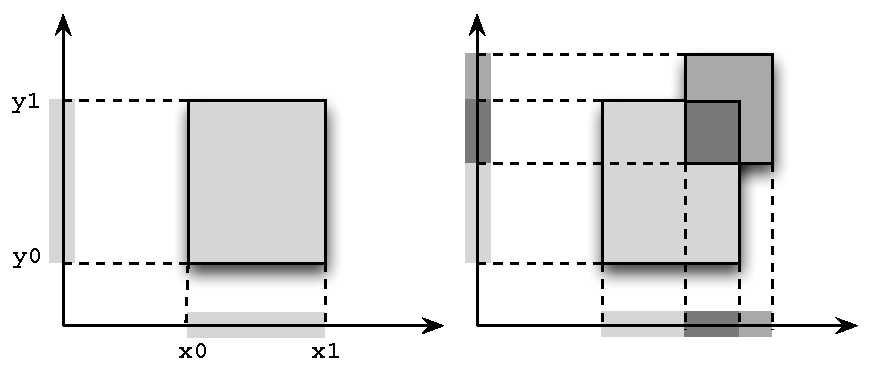
\includegraphics[width=0.9\baseimgwidth]{imgs/segments2DG}
\caption{from left to right: a graphic segment and the intersection of  two graphic segments.}
\label{fig:segment2D}
\end{center}
\end{figure}

%----------------------------------------------------------------
\subsection{Segment Generalization}
\label{segments}
%----------------------------------------------------------------
More generally, the notions of temporal and graphic segment can be extended to any dimension $n$.
A $n$-dimensional segment $s$ is defined as the cartesian product of $n$ intervals $s = i_1\times ... \times i_n$. 
When one of these intervals is empty, then $s$ is empty.

The intersection of $n$-dimensional segments is defined as:
\begin{equation}
\label{eq:segintersect}
s_1 \cap s_2 := (i_1 \cap j_1) \times ... \times (i_n \cap j_n)
\end{equation} 
where $s_1 = i_1 \times ... \times i_n$ et $s_2 = j_1 \times ... \times j_n$


%----------------------------------------------------------------
\subsection{Resource Segmentation}
\label{segmentation}
%----------------------------------------------------------------

% quel est la notion importante ici, resource or segmentation ????

By definition, a \emph{resource} is a non empty $n$-dimensional segment. 
The segmentation of a resource $R$, defined on a segment $S$, is a set of disjoined segments
$\displaystyle{\seg{R}=\{ s_1,..., s_p\}}$ all included in the resource:
\begin{equation}
\label{eq:segmdef}
\left\{
\begin{array}{l}
%	\forall s \in \seg{R} \quad s \cap S = s 			 \\
	\forall i \quad 1 \leq i \leq p \quad s \subseteq S \\
	\forall i, j \quad 1 \leq i \leq p,\quad 1 \leq j \leq p \quad \\
	 \hspace{2.9cm} i \ne j\ \Rightarrow\  s_i \cap s_j =  \emptyseg	 \\
\end{array}
\right.
\end{equation}

The segmentation \emph{domain} is defined as the union of its segments :
$$ \domaine(\seg{R}) = \bigcup_{i=1}^p s_i $$

Note that a segmentation is generally partial, it is not necessary a tessellation of the resource. % (see figure \ref


%----------------------------------------------------------------
\section{Mapping}
\label{resmap}

% Segment Mapping ? Discrete mapping ?

%----------------------------------------------------------------

A \emph{mapping} is a binary relationship between \emph{segmentations}, defined by a subset $M\subseteq \seg{R_{1}}\times \seg{R_{2}}$. We define the function $M^{+} : \seg{R_1} \rightarrow 2^{\seg{R_2}}$ that gives the set of segments from $R_{2}$ associated to a segment $s$ from $R_{1}$ :
\begin{equation}
\label{eq:mplus}
	M^{+}(s) :=\{ s' \in \seg{R_{2}}\ |\ (s,s') \in M\}
\end{equation}
 

Similarly we define the function $M^{-} : \seg{R_2} \rightarrow 2^{\seg{R_1}}$ that gives the set of segments from $R_{1}$ associated to a segment $s'$ from $R_{2}$.:
\begin{equation}
\label{eq:mmoins}
	M^{-}(s') :=\{ s \in \seg{R_{1}}\ |\ (s,s') \in M\}
\end{equation}

Mappings can catch any musical structure as shown by the example below. 
%musical structure is vague ...

%----------------------------------------------------------------
\subsection{Time to time mapping}\label{subsec:ttmap}

A \emph{time to time} mapping catch the overall music structure of a score and its relationship to the performance time. Consider the score as illustrated in figure \ref{fig:ex0-repeat}, which includes repeat bars. The relationship between the score time and the performance time can be described by the following relations set (assuming that the repeat section is played twice) : 
\maptab{0.8}{-3mm}{
( [0/1, 1/2[ ) & ( [0/1, 1/2[ )\\
( [1/2, 3/2[ ) & ( [1/2, 3/2[ )\\
( [1/2, 3/2[ ) & ( [3/2, 5/2[ )\\
( [3/2, 4/2[ ) & ( [5/2, 6/2[ )
}
where each line associates a score time segment to a performance time segment.
Time intervals are expressed as rational values denoting music time, where 1 is the whole note.
\begin{figure} %[htbp]
\begin{center}
	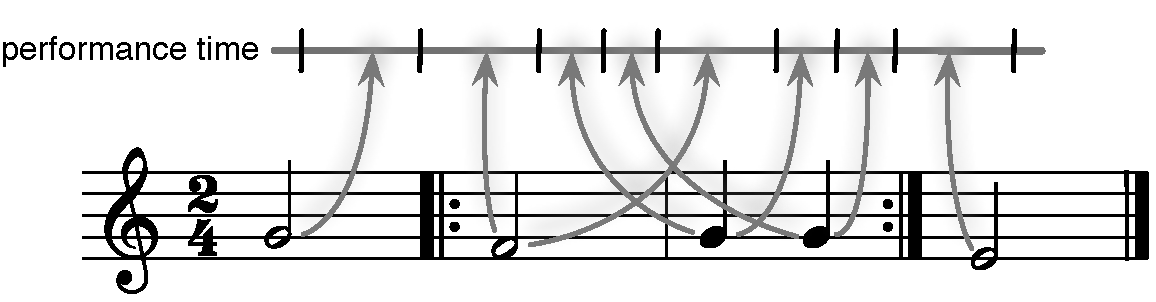
\includegraphics[width=0.9\baseimgwidth]{imgs/ex0-repeat2}
\caption{A music score including repeat bars: there is a non-bijective relationship between the notated and performance time.}
\label{fig:ex0-repeat}
\end{center}
\end{figure}

A time to time mapping is flexible enough to describe any musical structure, being not constrained to standard musical segmentation (e.g. measures). 


%----------------------------------------------------------------
\subsection{Mappings Composition}\label{subsec:compmap}
Composition of mappings is quite straightforward (figure \ref{fig:composition}):
using the mappings \\
\hspace*{2cm} $M_{1}\subseteq \seg{R_{1}}\times \seg{R_{2}}$ \\
\hspace*{1.3cm} and $M_{2}\subseteq \seg{R_{2}}\times \seg{R_{3}}$, \\
$M_1 \compose M_2$ is the mapping defined on  $\seg{R_{1}}\times \seg{R_{3}}$ by: 
\ifdefined \cmjversion
\begin{equation}
 (s,u) \in M_1 \compose M_2  \Leftrightarrow   
 \exists t \in \seg{R_2}\ |\ (s,t) \in M_1\ \land\ (t,u) \in M_2
\end{equation}
\else
\begin{align}
 (s,u) \in M_1 \compose M_2  \Leftrightarrow \nonumber \\
 \exists t \in \seg{R_2}\ |\ (s,t) \in M_1\ \land\ (t,u) \in M_2
\end{align}
\fi

\begin{figure} %[htbp]
\begin{center}
	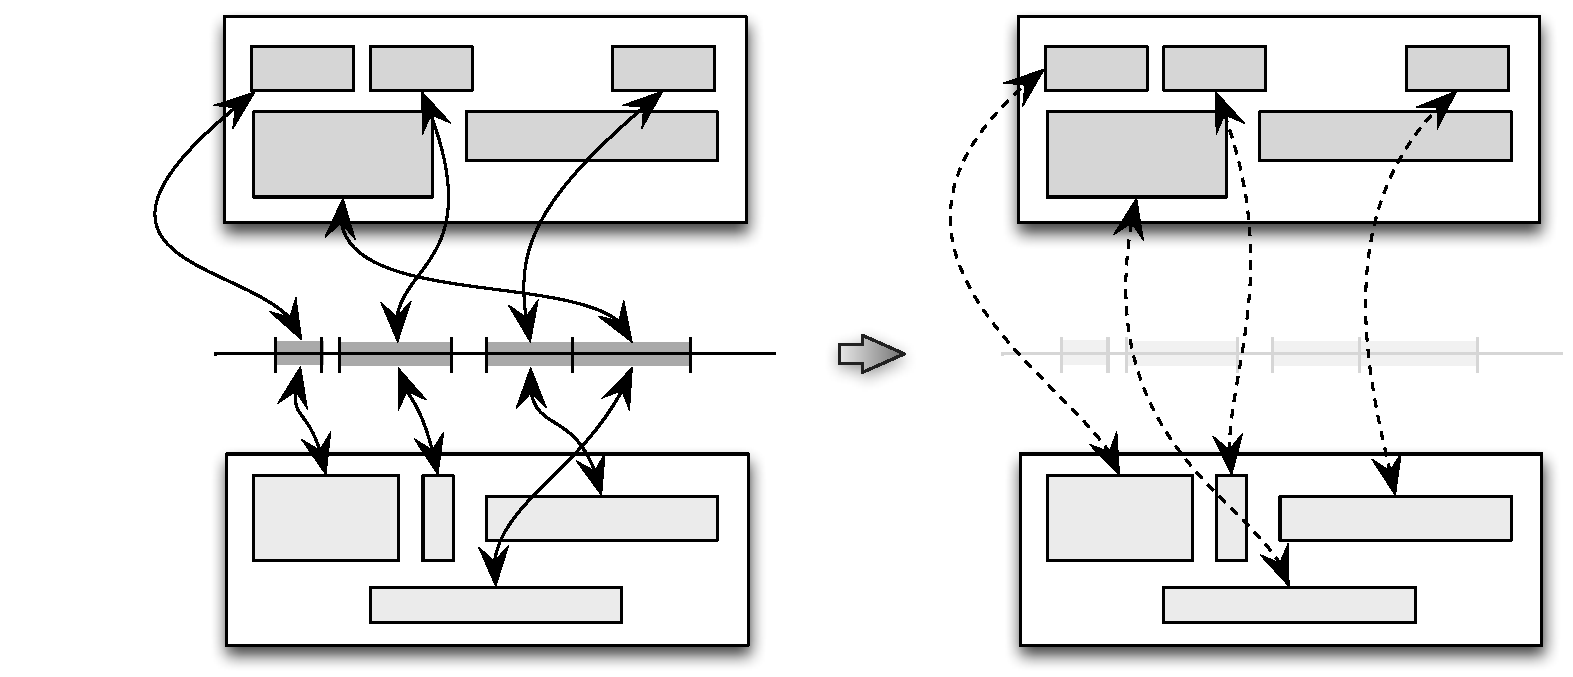
\includegraphics[width=0.9\baseimgwidth]{imgs/composition4}
\caption{Mappings composition.}
\label{fig:composition}
\end{center}
\end{figure}

Mappings composition allows to draw relationships between arbitrary segmentations, provided they have a relationship to a common space (e.g. the time space). This is illustrated in figure \ref{fig:composition}, where relationships between two graphic spaces are obtained from their relationships to the time space.

%----------------------------------------------------------------
\subsection{Time synchronization in the graphical space}\label{subsec:graphsync}

% This is an example of previous section ????

Mapping compositions can express time relationships in the graphical space. Let us consider the problem of a score and the graphical representation of its performance, as previously described. % in section \ref{sec:timetograph}. 
Figure \ref{fig:ex1-score} shows the different graphic segments of a score, annotated with the corresponding time segments, along with a graphic signal as a representation of a performance, also segmented in the graphic and time spaces.

Let $M_s\subseteq \seg{Score_{g}}\times \seg{Score_{t}}$ be the mapping between the score graphic and time segmentations.

\begin{figure} %[htbp]
\begin{center}
	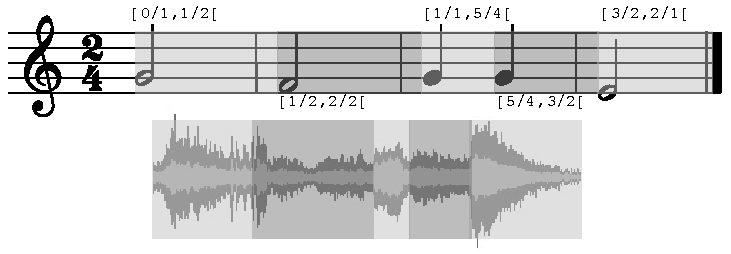
\includegraphics[width=0.9\baseimgwidth]{imgs/segmentation}
\caption{Graphic segments of a score and its performance displayed using grey levels and annotated with the corresponding time segments.}
\label{fig:ex1-score}
\end{center}
\end{figure}

Let $M_p\subseteq \seg{Perf_{t}}\times \seg{Perf_{g}}$ be the mapping between the performance time and graphic segmentationss.

The composition $M_s \compose M_p$ is a set of relationships from the score graphic space to the signal graphic space, directly expressing the time relationships of the two objects as illustrated in figure \ref{fig:ex1-sync}.

\begin{figure} %[htbp]
\begin{center}
	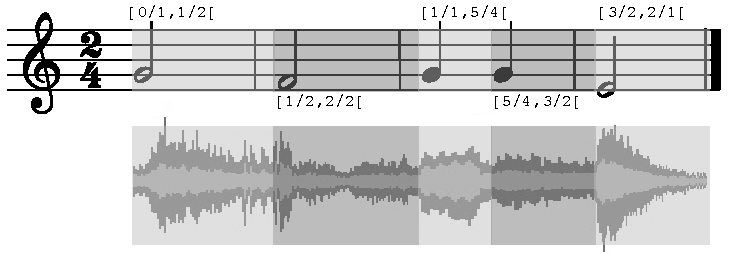
\includegraphics[width=0.9\baseimgwidth]{imgs/sync}
\caption{A score and its performance synchronized according to their time relationship using mappings composition.}
\label{fig:ex1-sync}
\end{center}
\end{figure}


%----------------------------------------------------------------
\section{\VDMapping}
\label{sec:vmap}
%----------------------------------------------------------------
We introduce the notion of \emph{\vdmapping}, that expresses relationships that are not explicitly described but that can be computed from a given mapping. 
For a relationship $(s,g) \in M$ a \emph{\vdmapping}\ describes the relationships of any segment $s' \subset s$. 

We first introduce the notions of intervals and segments \emph{varieties}. Next, we will define \emph{congruent varieties}, which provide for the ground for \vdmapping .


%------------------------------------------------------------
\subsection{Interval Variety}\label{sub:ivariete}

For  $\theta : [0,1] \rightarrow [0,1]$ and $I = [a, b [$, we name variety of $I$, the set of points $\variete(I,\theta)$ from $I$ defined by :
\begin{equation}
 \variete(I,\theta) = \left\{\ (1 - \theta(t)).a + \theta(t).b \ | \ t \in [0, 1[\ \right\}
\end{equation}

Intuitively, the variety of an interval expresses the relationship between this interval and its variety using a function $\theta$ defined on $[0, 1[$.

%------------------------------------------------------------
\subsection{Segment Variety}\label{sub:segvariete}

The variety of a segment generalizes the variety of an interval to a list of intervals.
It is defined as the list of the varieties of each interval.\\
Considering a segment $S = (i_1, ... , i_n)$ and $\Theta : n \to (\theta_1, ... , \theta_n)$, the variety $\variete(S, \Theta)$ of $S$ is defined as:
\begin{equation}
 \variete(S, \Theta) = (\variete(i_1,\theta_1), ... , \variete(i_n, \theta_n))
\end{equation}

More generally, we define the variety $\variete(S, \Theta^m)$ for $m \neq n$.
\begin{equation}
\begin{cases}
\variete(S, \Theta(m)) = (\variete(i_1,\theta_1), ... , \variete(i_m, \theta_m), \\
\hspace{2cm} \variete(i_{m+1}, \identite), ..., \variete(i_n, \identite))
, \quad m < n \\
\variete(S, \Theta(m)) = (\variete(i_1,\theta_1), ... , \variete(i_n, \theta_n)), \quad m > n
\end{cases}
\end{equation}
It consists respectively in the extension of the list of functions $\theta_i$ from the dimension $m$ to $n$ using the identity function and to the reduction of the list of functions $\theta_i$ to the dimension $n$.

Generally, we will note  $\variete(S, \Theta)$ to refer to a variety of $S$, whatever the dimensions of $S$ and $\Theta$.


%------------------------------------------------------------
\subsection{Congruent varieties}\label{sub:simvariete}

Two varieties $\variete(S, \Theta)$ and $\variete(T, \Theta')$  are said congruent when $\Theta = \Theta'$.\\ 
We will use the notation $\variete(S, \Theta) \semblable \variete(T, \Theta')$ to express congruence.

Intuitively, congruent varieties express the fact that the segments proportions and position relationships are equal. It also provides information about the relations between points enclosed in congruent varieties. 

Let's consider 2 time intervals $I=[t_1, t_2[$ and $I'=[t_1',t_2'[$ and a relationship between $I$ and $I'$. Congruent varieties $\variete(I, \Theta)$ and $\variete(I', \Theta)$ express how we go through $I'$ when we go through $I$ since 
\[
(1 - \theta(n)).t_1 + \theta(n).t_2 = (1 - \theta(n)).t_1' + \theta(n).t_2' \ | \ n \in [0, 1[
\]
In particular, the relationship between points from $I$ and $I'$ is deduced by linear interpolation when $\theta=\identite$.

The introduction of a function $\theta \ne id$ to go through a segment corresponds to the typical case of an accelerando, where the acceleration is a not a linear function of time.


%------------------------------------------------------------
\subsection{\VDMapping\ Definition} \label{subsec:vmap}
We can now define the \vdmapping .
For any mapping $M\subseteq \seg{R_1}\times \seg{R_2}$, we associate a mapping between varieties called \emph{\vdmapping}\ associated to $M$ as follows:
\begin{equation}
M_{\variete}^+(\variete(s,\theta))  = \{ \variete(s',\theta)\ |\ (s, s') \in M \}
\end{equation}

\begin{equation}
M_{\variete}^-(\variete(s',\theta)) = \{ \variete(s,\theta)\ |\ (s, s') \in M \}
\end{equation}


In other words: when two segments are in relationship, then their congruent varieties are also in relationship (figure \ref{fig:vmapping}).

\begin{figure} %[htbp]
\begin{center}
	\psfrag{V(s,t)}{$\variete(s,\Theta)$}
	\psfrag{V(g,t)}{$\variete(g,\Theta)$}
	\psfrag{s}{$s$}
	\psfrag{g}{$g$}
	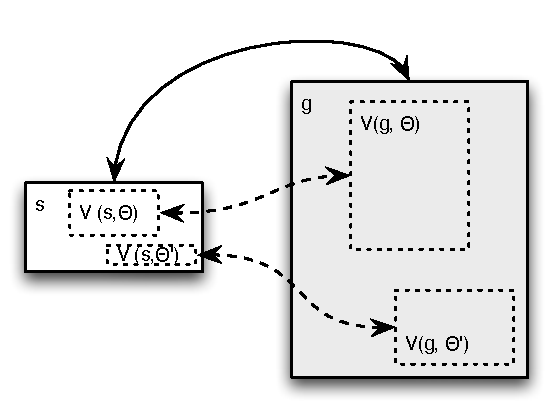
\includegraphics[width=0.7\baseimgwidth]{imgs/vmapping}
%\caption{Virtual mapping denoted by the dotted line, between congruent varieties.}
\caption{According to the relation between the segments $s$ and $g$, the continuous mapping expresses relations between included segments using congruent varieties, denoted by the dotted lines.}
\label{fig:vmapping}
\end{center}
\end{figure}

%------------------------------------------------------------
\section{Segmentations refinement}
\label{subsec:isegm}

The mappings composition makes explicit relationships when the resources share the same intermediate segmentation (for example, identical segmentation of the time space). 
In practice, we often have different segmentations of identical spaces, which cannot be \emph{composable} (figure \ref{fig:compo}), although we have the intuition that such relationship could be defined. To solve this problem, we build a common segmentation by \emph{refinement}.

\begin{figure} %[htbp]
\begin{center}
	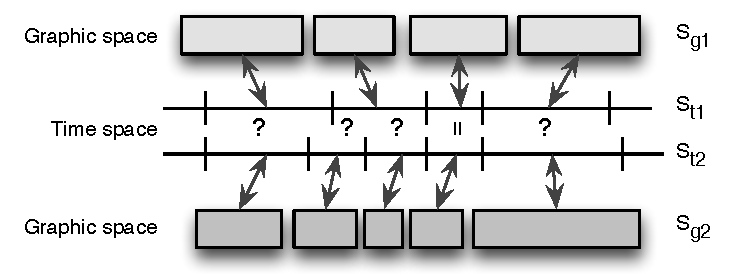
\includegraphics[width=0.9\baseimgwidth]{imgs/composition3}
\caption{Different segmentations of the same temporal space preventing the composition of the mappings $M \subseteq S_{g1} \times S_{t1}$ and $M' \subseteq S_{t2} \times S_{g2}$.}
\label{fig:compo}
\end{center}
\end{figure}


Let's consider a resource $R$ and two segmentations $S$ and $S'$ defined on $R$, we define the relationship denoted $\raff$ to express that $S'$
is \emph{finer} than $S$ (every segment of $S'$ is included in a segment of $S$) :
$$ S' \raff S \quad  \Leftrightarrow  \quad \forall s' \in S' \quad \exists\ s \in S \quad s' \subset s $$
This relationship could be viewed as a variety of $s$:
\begin{align}
 S' \raff S \quad  \Leftrightarrow  \quad \forall s' \in S' \nonumber \\
 \exists\ (s,\theta) \in S \times \fvariete  \quad s' =\variete(s,\theta)
\end{align}

Note that two segmentations $S_1$ and $S_2$ defined on the same resource $R$ have always a common partial refinement $S$ on their intersection when this intersection is not empty (figure \ref{fig:isegm}) satisfying:
\[
\begin{cases}
\domaine(S) = \domaine(S_1) \cap \domaine(S_2) \\
S \raff S_1\ \land\ S \raff S_2 \\
\end{cases}
\]

\begin{figure} %[htbp]
\begin{center}
	\psfrag{S1}{$S_1$}
	\psfrag{S2}{$S_2$}
	\psfrag{S}{$S \raff S_1\ \land\ S \raff S_2$}
	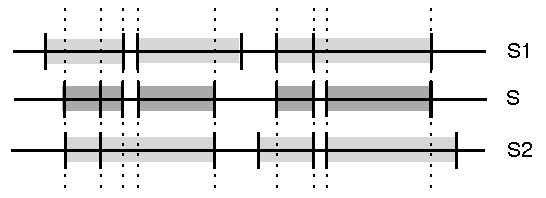
\includegraphics[width=0.9\baseimgwidth]{imgs/segintersect}
\caption{The refinement $S$ of the two segmentations $S1$ and $S2$.}
\label{fig:isegm}
\end{center}
\end{figure}

The refinement common to two segmentations $S_1$ et $S_2$ may also be expressed as varieties:
\begin{align}
S \raff S_1\ \land\ S \raff S_2  \quad \Leftrightarrow  \quad \forall s \in S  \nonumber\\
\exists\ (s_1,\theta) \in S_1 \times \fvariete \nonumber\\
\quad \exists\ (s_2, \delta) \in S_2 \times \fvariete \nonumber\\
\quad s = \variete(s_1,\theta) = \variete(s_2,\delta)
\end{align}


%------------------------------------------------------------
\subsection{Example 1: A sliding window with a time dimension}
\label{sub:window}

A basic use case of \vdmapping\ and refinement consists in a sliding window with a time dimension which could serve analysis or performance purposes. The window is aligned to a score to indicate the current time position and time extend as shown in figure \ref{fig:ex2}, where the score time and graphic segmentations are as illustrated in figure \ref{fig:ex1-score}. The window duration is $1/2$ (a half note) and its current time position ($3/4$) lies in the middle of the time segment $S_t=[1/2, 1/1[$.

\begin{figure} %[htbp]
\begin{center}
	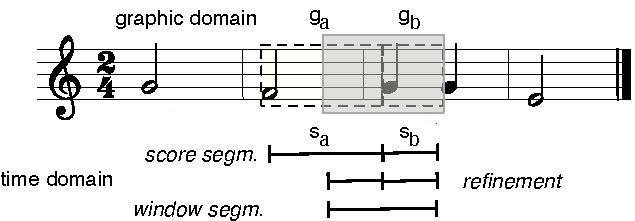
\includegraphics[width=0.9\baseimgwidth]{imgs/ex2-2}
\caption{A window aligned to a score at date 3/4. Its duration is 1/2 (a half note). The corresponding time segments are shown with their refinement.}
\label{fig:ex2}
\end{center}
\end{figure}

The score time segmentation in the window neighborhood is $S=\{s_a=[1/2, 1/1[\quad s_b=[1/1, 5/4[\}$ and the window time segmentation is $C=\{[3/4, 5/4[\}$. We assume that we have the following time to gaphic mapping:
\texttt{\begin{center}
\begin{tabular}{r@{ \lra }l}
 $s_a$ & \ $g_a$ \\
 $s_b$ & \ $g_b$ 
\end{tabular}
\end{center}
}
where $g_a$ and $g_b$ are gaphic segments.\\
The segmentation $S_R=\{[3/4, 1/1[\quad[1/1, 5/4[\}$ is a refinement of both $S$ and $C$. 

Using a function $\theta=id$ (i.e. a linear interpolation), the continuous mapping tells us that the first half of the window $[3/4, 1/1[$ is mapped to the second half of the score $g_a$ graphic segment and the second half of the window 
$[1/1, 5/4[$ is mapped to the $g_b$ graphic segment.

Using mappings and \vdmapping s turns out to be a very convenient way to synchronize any object to a score without taking care of the score layout (e.g.  without the need to detect whether there is a line break in the middle of my objet). Any object can be expressed in the temporal domain, the mapping and \vdmapping\ taking care of potential sub-segmentation with every corresponding graphic segments.


%------------------------------------------------------------
\subsection{Example 2: Multiples Segmentations in Sound and Gesture Signal Representations}

At the beginning of the paper \ref{sec:timetograph}, we presented an example where gesture and sounds signals were separately segmented and linked to the score (Fig.   \ref{fig:gmapping-gesture-sound}). We can see now how our general formalism can handle such a complex case. First, a comparison between Figure \ref{fig:gmapping-gesture-sound} and Figure \ref{fig:compo} reveals clearly that the segmentation refinement is appropriate to formalize the different segmentations such as the gestural and sound segmentation, that operates in the on the same performance time. 
%This case can be handled directly using the segmentation refinement formalism described above. Figure \ref{fig:gmapping-gesture-sound} can indeed be seen as a direct illustration of Figure \ref{fig:compo}, where two different segmentations are operated on the same performance time. 



\section{Implementation}
The mapping formalism has been implemented as a C++ library. It is part of the INScore open source project \footnote{http://inscore.sf.net} where it provides time synchronization in the graphic space. The system automatically aligns and stretches synchronized objects to the corresponding score location using this library, to easily produce the kind of results illustrated in figure \ref{fig:ex1-sync}. Examples are given in \cite{Fober:10c}\cite{Fober:12a}.


\section{Conclusion}
We have proposed a simple formalism to describe relationships between segments. This formalism is general since it does not rely in any way on the segments content and semantic. As such, it has musical applications in the graphic domain of the score but also in the gestural or audio domains and allows to create links that would be otherwise complex to express. It also includes a formal description of operations that gives a high flexibility to the way relationships can be described, including how the inner space of a segment relates to another segment space.

%This formalism has been implemented in an open source software, representing a first example of the uses of this formalism that should benefit the music computation community.


%=============================================================
%\vspace{4mm}
\section{Acknowledgments}
This research has been made in the framework of the Interlude project [ANR-08-CORD-010]. It has been extended in the Inedit project [ ANR-12-CORD-0009-03]. Both projects have been funded by the Agence Nationale pour la Recherche.


%\begin{dgroup*}
%\begin{dmath*}
%S \raff S_1\ \land\ S \raff S_2  \ \Leftrightarrow  \ \forall s \in S \\ \exists\ (s_1,\theta) \in S_1 \times \fvariete\ \exists\ (s_2, \delta) \in S_2 \times \fvariete \quad s = \variete(s_1,\theta) = \variete(s_2,\delta)
%\end{dmath*}
%\end{dgroup*}


%\section{Applications}
%
%The formalism described above is independent of the type of resources we want to manipulate and of the dimensions of these resources as well. It is expected to be simple and powerful enough to satisfy the needs of a great variety of applications.
%Taken from the music domain, two examples of applications are provided below.
%
%\subsection{Graphic to time mapping}
%
%
%
%
%
%\subsection{Gesture to sound mapping}
%
%\section{Discussion/Conclusion}


\ifdefined \acmversion
\bibliographystyle{unsrt}
\fi

\ifdefined \cmjversion
\bibliographystyle{cmj}
\fi

\ifdefined \mamversion
\bibliographystyle{tMAM}
\fi

\bibliography{references}

\end{document}